\documentclass[12pt]{article}

\usepackage{sbc-template}

\usepackage{graphicx,url}

\usepackage[portuguese, ruled, linesnumbered]{algorithm2e}
\usepackage[brazil]{babel}   
%\usepackage[latin1]{inputenc}  
\usepackage[utf8]{inputenc}  
% UTF-8 encoding is recommended by ShareLaTex

     
\sloppy

\title{Problema da Seleção de Atividades}

\author{Gabriel O. Machado\inst{1} }


\address{Departamento de Computação -- Universidade Federal de Ouro Preto
  (UFOP)\\
  Campus Universitário Morro do Cruzeiro  -- 35400-000  --  Ouro Preto -- MG -- Brasil
}

\begin{document} 

\maketitle

\begin{abstract}
	This assignment describes three different solutions for the Activity Selection Problem. One using a greedy solution, 
	another one by dynamic programming and a third one by Backtracking.
	At the end, the three results and running time are compared.
\end{abstract}
     
\begin{resumo} 
	Este trabalho descreve os detalhes da implementação do problema da seleção de atividades, 
	usando para tal uma solução através de algoritmos gulosos, outra solução por programação dinâmica
	e uma terceira que faz uso da técnica de Backtracking.
	Ao final são comparados os resultados e tempos de execução das três técnicas.
	
\end{resumo}


\section{Introdução}



\section{Método Guloso} \label{sec:guloso}

Os métodos gulosos são um conjunto de métodos que fazem uso da heurística da melhor solução local em cada etapa de execução. Por conta desta característica, não garantem a solução ótima de um problema.

Para que a solução gulosa apresente uma solução ótima, deve possuir a característica de que cada escolha gulosa contenha uma solução ótima para o problema proposto, mostrando assim que o restante do problema também possui uma solução ótima.

Neste trabalho, a implementação ótima foi realizada através do algoritmo abaixo:

 \begin{algorithm}[H]
   \SetAlgoLined
   \Entrada{$A$} 
   \Saida{Array contendo número máximo de atividades compatíveis entre si}
   \Inicio{
   $A(0) = 0$ \\
    \Para{cada $u \in A$}{
   $\sigma(S)\leftarrow \sigma(S)+\textsc{Backtrack}(u,\eta,W,U)$\\
     }
   }
   \Retorna{$\sigma(S)$}
   \label{alg1}
   \caption{\textsc{Seleção de Atividades}}
 \end{algorithm}


\section{Programação Dinâmica}


\section{Backtracking}

Section titles must be in boldface, 13pt, flush left. There should be an extra
12 pt of space before each title. Section numbering is optional. The first
paragraph of each section should not be indented, while the first lines of
subsequent paragraphs should be indented by 1.27 cm.

\subsection{Subsections}

The subsection titles must be in boldface, 12pt, flush left.

\section{Figures and Captions}\label{sec:figs}


Figure and table captions should be centered if less than one line
(Figure~\ref{fig:exampleFig1}), otherwise justified and indented by 0.8cm on
both margins, as shown in Figure~\ref{fig:exampleFig2}. The caption font must
be Helvetica, 10 point, boldface, with 6 points of space before and after each
caption.

\begin{figure}[ht]
\centering
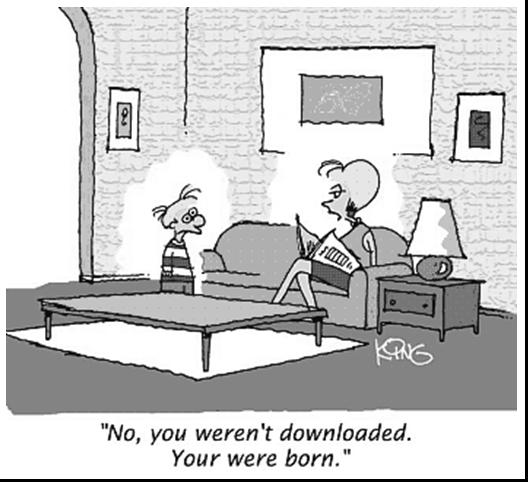
\includegraphics[width=.5\textwidth]{fig1.jpg}
\caption{A typical figure}
\label{fig:exampleFig1}
\end{figure}

\begin{figure}[ht]
\centering
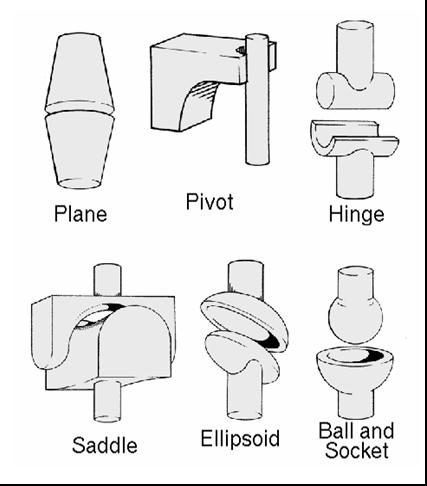
\includegraphics[width=.3\textwidth]{fig2.jpg}
\caption{This figure is an example of a figure caption taking more than one
  line and justified considering margins mentioned in Section~\ref{sec:figs}.}
\label{fig:exampleFig2}
\end{figure}

In tables, try to avoid the use of colored or shaded backgrounds, and avoid
thick, doubled, or unnecessary framing lines. When reporting empirical data,
do not use more decimal digits than warranted by their precision and
reproducibility. Table caption must be placed before the table (see Table 1)
and the font used must also be Helvetica, 10 point, boldface, with 6 points of
space before and after each caption.

\begin{table}[ht]
\centering
\caption{Variables to be considered on the evaluation of interaction
  techniques}
\label{tab:exTable1}
\smallskip
\begin{tabular}{|l|c|c|}
\hline
& Value 1 & Value 2\\[0.5ex]
\hline
&&\\[-2ex]
Case 1 & 1.0 $\pm$ 0.1 & 1.75$\times$10$^{-5}$ $\pm$ 5$\times$10$^{-7}$\\[0.5ex]
\hline
&&\\[-2ex]
Case 2 & 0.003(1) & 100.0\\[0.5ex]
\hline
\end{tabular}
\end{table}

\section{Images}

All images and illustrations should be in black-and-white, or gray tones,
excepting for the papers that will be electronically available (on CD-ROMs,
internet, etc.). The image resolution on paper should be about 600 dpi for
black-and-white images, and 150-300 dpi for grayscale images.  Do not include
images with excessive resolution, as they may take hours to print, without any
visible difference in the result. 

\bibliographystyle{sbc}
\bibliography{sbc-template}

\end{document}
